\documentclass[a4paper,11pt]{article}
\usepackage{epsfig}
\usepackage{amsmath}
\usepackage{amsfonts}
\usepackage{amssymb}
\usepackage{url}
\usepackage{hyperref}
\usepackage{color}

\textheight=24cm
\textwidth=16cm
\widowpenalty=5000
\topmargin=-2cm
\evensidemargin=-.5cm
\oddsidemargin=-.5cm
\hsize=17cm
\vsize=16cm
\hoffset=0.7cm
\voffset=1.5cm
\parindent 1em

\newcommand{\DocGeneralVersion}{{\bf v2.0}}
\newcommand{\CurrentDate}{March 2011}
\newcommand{\bverb}{\begin{verbatim}}
\newcommand{\everb}{\end{verbatim}}
\newcommand{\crp}{{\tt CRPropa}}
\newcommand{\sophia}{{\tt SOPHIA}}
\newcommand{\sibyll}{{\tt SIBYLL}}
\newcommand{\ROOT}{{\tt ROOT}}
\newcommand{\cfitsio}{{\tt CFITSIO}}
\newcommand{\comment}[2]{\textcolor{blue}{{\bf #1: }#2 }}

\def\arcsec{$''$}
\def\arcmin{$'$}
\newcommand{\meV}{{\rm meV}}
\newcommand{\eV}{{\rm eV}}
\newcommand{\keV}{{\rm keV}}
\newcommand{\MeV}{{\rm MeV}}
\newcommand{\GeV}{{\rm GeV}}
\newcommand{\TeV}{{\rm TeV}}
\newcommand{\PeV}{{\rm PeV}}
\newcommand{\EeV}{{\rm EeV}}
\newcommand{\erg}{{\rm ergs}}
\newcommand{\Mpc}{{\rm Mpc}}
\newcommand{\kpc}{{\rm kpc}}
\newcommand{\pc}{{\rm pc}}
\newcommand{\cm}{{\rm cm}}
\newcommand{\km}{{\rm km}}
\newcommand{\muG}{\mu{\rm G}}
\newcommand{\mG}{{\rm mG}}
\newcommand{\G}{{\rm G}}
\newcommand{\s}{{\rm s}}
\newcommand{\yr}{{\rm yr}}
\newcommand{\sr}{{\rm sr}}
\newcommand{\Hz}{{\rm Hz}}
\newcommand{\nubar}{\bar{\nu}}
\newcommand{\GS}{\textcolor{red}}
\newcommand{\PS}{\textcolor{blue}}
\newcommand{\LM}{\textcolor{magenta}}
\newcommand{\AvV}{\textcolor{green}}



\begin{document}

\pagestyle{empty}

\begin{titlepage}
\Huge\bf
\vspace*{1cm}
\centerline{The}
\centerline{\crp\ framework}
\vspace{1cm}
%\centerline{\epsfig{file=Auger_logo.ps,height=6cm}}
\vspace{1cm}

\begin{center}
{\huge \bf A numeric tool to study propagation effects on UHECRs and
their secondaries in the Local Universe}

\vspace{1.cm}

{\LARGE \bf Version \DocGeneralVersion}\\[5mm]
\large \today

%\vspace{2cm}
\url{http://crpropa.desy.de}\\

\vspace{3cm}

J\"org Kulbartz,  \href{mailto:jkulbart@mail.desy.de}{\nolinkurl{jkulbart@mail.desy.de}}\\
Universit\"at Hamburg

Nils Nierstenh\"ofer, \href{mailto:Nierstenhoefer@physik.uni-wuppertal.de}{\nolinkurl{Nierstenhoefer@physik.uni-wuppertal.de}}\\
Universit\"at Wuppertal

G\"unter Sigl, \href{mailto:guenter.sigl@desy.de}{\nolinkurl{guenter.sigl@desy.de}}\\
Universit\"at Hamburg

Luca Maccione, \href{mailto:luca.maccione@lmu.de}{\nolinkurl{luca.maccione@lmu.de}}\\
LMU \& MPP, M\"unchen

Peter Schiffer, \href{mailto:peter.schiffer@desy.de}{\nolinkurl{peter.schiffer@desy.de}}\\
Universit\"at Hamburg

Arjen van Vliet, \href{mailto:arjen.rene.van.vliet@desy.de}{\nolinkurl{arjen.rene.van.vliet@desy.de}}\\
Universit\"at Hamburg

Former authors:\\
\'Eric ARMENGAUD, \href{mailto:armengau@in2p3.fr}{\nolinkurl{armengau@in2p3.fr}} \\
Tristan BEAU, \href{mailto:beau@in2p3.fr}{\nolinkurl{beau@in2p3.fr}}\\
APC / IAP - Paris, France.
\vspace{1cm}

\end{center}


\end{titlepage}

\section*{Overview}
CRPropa is a publicly available code to study the propagation of UHE-nuclei up to iron taking into account: pion production, photodisintegration and energy losses by pair production of all relevant isotopes in the ambient low energy photon fields as well as nuclear decay. CRPropa can model the deflection in intergalactic magnetic fields, the propagation of
secondary electromagnetic cascades and neutrinos for a multitude of scenarios for different source distributions and magnetic environments. It enables the user to predict the spectra of UHECR (and of their secondaries), their composition and arrival direction distribution.

In this documentation you will find information about:
\begin{description}
\item[What \crp\ can do.] We present general features of
the framework, and the current possibilities they offer. We also briefly discuss possible future improvements.
\item[Installing the software.] We describe the needed dependencies and complementary packages, as well as the required steps to get to compilation and installation of the software.
\item[Understanding the details of the software] The architecture of \crp\ and of the external modules are presented, as well as some technical details.
\item[Using the input/output.] We describe the input and output format in detail and we discuss the relevant options that should be set by the user. We also present plotting routines that can be used to acquire competence with the code. 
\end{description}


This manual focuses on technical details which the user needs to know to work with CRPropa. Details on the treatment of particle- and nuclear physics as well as cosmology within CRPropa can be found in the accompanying paper \cite{crp2paper}.

\cleardoublepage
\tableofcontents
\cleardoublepage
\pagenumbering{arabic}
\pagestyle{plain}

\section{Description of \crp}

\subsection{Presentation}

\crp\ is a numerical tool designed to study the propagation of charged
UHECRs in our ``Local environment'', as well as their secondary $\gamma$-rays and neutrinos.

While propagating in the intergalactic medium (IGM), charged UHECRs are deflected by intergalactic magnetic fields and interact with radiation fields through essentially photopion production and pair production reactions as well as photodisintegration of nuclei. Such interactions have typical mean free paths $\gtrsim$ a few Mpc, and the energy lost in one interaction is typically of the order of a few percent or up to 20\% of the initial particle energy in case of nucleons. The energy loss for nuclei in photodisintegration reactions can be even larger, up to 67\%. Additionally, primary nuclei can lose nucleons in these interactions thereby changing their type. Given the accuracy of present day experiments, like the Pierre Auger Observatory (PAO), the propagation of charged UHECRs must be described within a Monte Carlo approach.

The main observational properties of UHECRs are their energy spectrum, their mass composition and their arrival directions, which in turn are determined by various physical properties of the IGM and of the UHECR sources, which we list below:

%The use of such a software is needed in order to interpret the
%highest-energy data from UHECR observatories such as Auger. The
%observable properties of UHECRs, namely their spectrum, composition
%and anisotropies depend on various parameters, which we briefly remind
%to the reader here:

\begin{description}
\item[The source properties and distribution.]
The sources of charged UHECRs are currently unknown, but might for instance be active galactic nuclei (AGNs) or gamma ray bursts (GRBs). Independent of their true nature, the most important ingredient is their injection spectra and their distribution in the local universe. In particular, the ``end of the spectrum'' of UHECRs might be dominated by nearby sources. The spectrum and
anisotropies at these energies depend on the exact source configuration.

\item[The interactions with low-energy backgrounds.]
Charged nuclei undergo pair and pion production, and therefore generate secondary neutrinos and electromagnetic cascades whose detection might provide important hints to the sources of UHECRs, as has already been the case at lower energy. Additionally nuclei photodisintegrate on low energy backgrounds. Subsequently unstable nuclei produced in the aforementioned interactions decay.

\item[The deflections in magnetic fields.]
Although they are very poorly known, magnetic fields might play a significant role even for
the highest energy particles, by deflecting their propagation direction and increasing the
mean path from the source to the observer.

\item[The composition of the injected cosmic rays.]
The composition of UHECRs at injection influences the reactions of cosmic rays in low energy photon backgrounds as well as the deflections of their trajectories.
\end{description}

%Thanks to its unprecedented statistics at the highest energies, the
%Pierre Auger Observatory might be able to do some kind of charged
%particle astrophysics. 
\crp\ is meant to model these relevant processes as accurately as possible in order to understand the details of UHE sources, as well as their possible neutrino and gamma counterparts at lower energies. A description of the physics taken into account by the previous version of \crp\ can be found in~\cite{crp_paper}.


%\subsection{What \crp\ can do}
\subsection{\crp\ features}

%Here we give examples of what this framework can already do, what are
%its limitations and what are possible future improvements.
Here we give examples of what this framework can do at the moment and of what are its limitations. 

\begin{description}
\item[General features.] \crp\ calculates the energy losses of UHECRs in the energy range of $7\cdot 10^{16}-10^{22}\cdot A$~eV where $A$ is the mass number of the nucleus. For the energy losses it takes into account photopair production, photopion production and additionally photodisintegration and the possible decay of nuclei. Additionally it calculates neutral secondaries as well as daughter nuclei produced in nuclear reactions. 

\item[1D propagation.] In 1D, we can study the interactions of protons and nuclei injected from a given source distribution to an observer in the absence of magnetic field deflections. The source distribution can be any continuous function (possibly including redshift evolution) or discrete list of sources. We can also follow the secondary ``cosmogenic'' neutrinos as well as the electromagnetic cascades down to 10 MeV. A possibly inhomogeneous transverse magnetic field can be taken into account in the cascade modeling, as well as various IR and radio backgrounds. In 1D additionally redshift effects are taken into account.

\item[3D propagation.] In 3D, we can follow the propagation of protons and nuclei injected from sources in the presence of magnetic field deflections. This might be especially relevant for heavy nuclei, which are deflected more compared to protons, and for estimating electromagnetic cascades. Because of deflections, the total propagation time of a particle cannot be determined {\it a priori}, knowing the distance between its source and the observer. Therefore, redshift becomes an ill-defined concept and no redshift effect is included. As a further consequence, and also due to computational requirements, the simulation is performed typically into a box of $\sim$ 100 Mpc (linear) size, which is then replicated identically according to propagation requirements, assuming periodic boundary conditions at the interface between two boxes. In this sense, 3D propagation can only be ``local''. Any magnetic field grid  can be given as input, and its ``coordinate'' system is taken as the simulation box of \crp. Sources can be specified from a continuous density or using a discrete list of source coordinates. The simulation can follow ``full trajectories'', or record ``events''. The detection of events is of course possible only if observers are specified. Observers are typically spheres of a given radius at a given location. In case the user is interested in UHECRs at production from a given source (e.g.~a galaxy cluster), then an observer can be defined as a large sphere around the given single source.

\item[Propagation of secondary neutrinos and $\gamma$-rays.] Secondary neutrinos and/or electromagnetic cascades can be followed and recorded by the observers, both in 1D and 3D. The same magnetic field as used for nuclei deflections is used to model the cascades (whose propagation is however considered as rectilinear). We can therefore easily study the full ``multi-messenger'' spectrum of possible nearby UHECR sources.
\end{description}

Thanks to the modular implementation of the framework, it should be quite easy for 
the skilled user to add modules that allow to extend the possibilities of the code.

\subsection{Planned improvements}

\begin{itemize}
\item It is not possible to take into account redshift effects in the 3D propagation model given the present structure of the code, as we do not know in advance the redshift of a given source due to the time delays induced by deflections as well as the periodic boundary conditions. Therefore at the moment we can only model the 3D propagation of UHECRs and their secondaries in the ``local'' Universe, typically at distances below 1 Gpc. We are however looking into a way to approximate the redshift effects after the detection of the UHECR, when the redshift of the source is known.
\item Trajectories of UHECRs are also deflected due to the presence of galactic magnetic fields. Therefore, an interface with galactic deflection codes is planned.
\item Allowing for non-regular, AMR grids for the extragalactic magnetic fields seems also an important feature to be added in the future.
\item We also plan to allow for arbitrary dependence of the IR background on redshift.
\item UHECRs at low energy ($E \lesssim 1$~EeV) can in some situation more efficiently be described in terms of diffusion rather than ballistic propagation in a tangled magnetic field. Extension to the diffusive regime for trajectories at low energy is therefore planned.
\end{itemize}

%  \subsection{What \crp\ cannot do now... but will be considered for the future}
%  \begin{description}
%  \item[Considered] It is not possible to take into account redshift effects in the
%  3D propagation model given the present structure of the code, as we do not know in advance the redshift of a
%  given source due to the time delays induced by deflections as well as the
%  periodic boundary conditions. Therefore we can only model the 3D
%  propagation of UHECRs and their secondaries in the ``local'' Universe,
%  typically at distances below 1 Gpc. However, redshift effects in 3D could in principle be taken into account in a backward (in time) propagation, or in a 4-D approach.
%  
%  \item[Planned] Trajectories of UHECRs are also deflected due to the presence of galactic magnetic fields. Therefore, an interface with galactic deflection codes is planned.\\ Allowing for non-regular, AMR grids for the extragalactic magnetic fields seems also an important feature to be added in the future. \\We also plan to allow for arbitrary dependence of the IR background on redshift. \\UHECRs at low energy ($E \lesssim 1$~EeV) can in some situation more efficiently described in terms of diffusion rather than ballistic propagation in a tangled magnetic field. Extension to the diffusive regime for trajectories at low energy is therefore planned.
%  \end{description}

%\paragraph{Basic description of the modules}

\section{Technical details}
\crp\ is a C++ code, which uses some external modules. The C++ standard
template library is used, as well as the high energy physics library
CLHEP (for random numbers, vector transformations, the unit system,
etc.). The interactions of nuclei with low energy radiation backgrounds are handled with the \sophia~event generator, while interactions with the IGM gas are described by \sibyll. Both codes are written in FORTRAN. 
The propagation of electromagnetic cascades is calculated by DINT (written in C). Additionally some functions of \ROOT\ \cite{root} and FFTW \cite{FFTW05} are used.

In order to run \crp\ the user has to provide a configuration file. The configuration files must be in XML format, and are handled with the TinyXML library \cite{tinyxml}. The output files can be written in ASCII, FITS or ROOT, and therefore the \cfitsio~and \ROOT~library are required.

\subsection{Installing the code}

\crp\ uses the following modules: DINT~\cite{Lee:1996fp}, \sophia~\cite{sophia}, \sibyll~\cite{Ahn:2009wx}, TinyXML~\cite{tinyxml}, \cfitsio~\cite{cfitsio}, CLHEP~\cite{clhep}, FFTW~\cite{FFTW05} and \ROOT~\cite{root}. Among them, DINT, \sophia, \sibyll~and TinyXML are included in the distribution, and CRPropa provides an helper script for installation of CLHEP and \cfitsio. \ROOT\ and FFTW need to be installed before the installation of CRPropa. In addition a working autotools enviroment including a working C/C++ and FORTRAN compiler and doxygen is needed for the installation. 
%Furthermore, if you want to be able to use ROOT output you must have a reasonably recent version of ROOT installed~\cite{root}.

The installation has been tested mostly on Linux and Darwin (Mac OS) platforms. The following steps should work (there is also a README file in the package):
\begin{itemize}
\item Untar the package using: \verb+tar -xvzf <package-filename>+
\item If you do not have the external modules \cfitsio~and CLHEP yet, run the script \\\verb+get_external.sh+. Warning: you need a lot of disk space (750 MB), mostly because of the size of the CLHEP library.
\item Install \ROOT \ and FFTW if necessary. 
\item Run autoreconf -ivf, ./configure (with options if needed: see the README file), and make. It will compile the DINT, \sophia, \sibyll, documentation (including Doxygen if you have it) and \crp\ packages in order.
\item Now the code is compiled, but you need to download the tabulated mean free paths needed by the photodisintegration routines. You can get them by running the script \verb+GetPDCrossSections.sh+. 
\item Run \verb+make install+ to install the code and to copy the needed cross section tables into the install directory.
\end{itemize}
%
A simulation can be started by running $<$path-to-CRPropa executable$>$/CRPropa $<$configuration-file.xml$>$. During the simulation, after all the parameters are initialized from the configuration file, individual particle trajectories are followed
one after another. Secondaries are added to a ``queue'' and are simulated after the end of the primary trajectory, before other particles are generated from the sources. The simulation stops after a given number of particles has been injected from the sources. 


%{\bf Remark: since CRPropa v1.3, a new option for ./configure is --with-root. You need to set this option in order to be able to use ROOT.}
\subsection{Concept of the code}
Within \crp\ we extensively use the object-oriented language C++. A full description of all available classes is described in the Doxygen-generated documentation. The base classes are virtual, so that they get (re)implemented by real classes depending on the physical situation that is simulated. As an example, the fundamental virtual class for sources is TSources, and the classes TContinuousSources and TDiscreteSources are actual implementations of this class. All the fundamental parameters of the simulation are instantiated in a TBasicParam and a TUniverse object. The \verb+main+ has the following simple structure:

{\small 
\begin{verbatim}
    TEveryThing lAll(argv[1]); // Configuration
    TBasicParam *lpBasic = lAll.Basic; // Basic parameters
    TUniverse   *lpUniv  = lAll.Univ; // Propagation environment

    QUEUE<TParticle*> lParts;          // List of particles to propagate
    TList1DPhotons lPhotons1D(lpUniv); // List of photons in the 1D case

    unsigned long lN = 0;
    while ( lN < lpBasic->N() ) { // Loop on trajectories
        lParts.clear();
        lParts.push_back( new TNucleus(lpUniv, &lPhotons1D) ); // inject nucleus
        lN++;
        while ( lParts.size() ) { // Loop on generated secondaries
            QUEUE<TParticle*>* lNewSet;
            lNewSet = lParts.back()->Propagate(lpBasic); // Propagation
            delete lParts.back();
            lParts.pop_back();
            lParts.insert(lParts.end(),lNewSet->begin(),lNewSet->end());
            lNewSet->clear();
        }
    }

    lPhotons1D.Propagate(lpUniv,lpBasic); // Propagate photons in the 1D case
\end{verbatim}
}

In 1D, a list of empty electromagnetic cascades, located at various redshifts, is created before the propagation of nuclei. The distribution along the line-of-sight of injected photons and pairs is populated during propagation of all injected nuclei, and the resulting transport equation with a continuous injection distribution is solved once at the end of the simulation. The advantage of this procedure, with respect to the propagation of each single injected secondary photon or pair, is a considerable gain of CPU time for electromagnetic cascades generated at large redshifts, while the limitation is that photon showers in 1D cannot be reweighted to a different CR injection spectrum.\label{1dphotons} In addition this approach can introduce an error if the step size of the primary UHECR is larger than the step size of the cascades. Therefore in 1D simulations with secondary photons the step size should not be larger than $1$~Mpc.

\subsection{Propagation Algorithm}\label{propAlgo}
Because of the very small mean free path of photodisintegration, especially for heavy nuclei, and the strongly varying decay lengths of unstable nuclei, it is necessary to use a propagation algorithm that is particularly efficient in dealing with the various length scales. We deal with this problem by determining the time until the next reaction of a UHECR takes place and then propagating the particle over this time step. After this time step the determined interaction takes place. 

The algorithm works as follows. 
Given the mean free path $\lambda_{i}$ for a given interaction channel of a given nucleus, where $i$ runs over all $N$ possible interaction and decay channels,
\begin{enumerate}  
\item The inverse total mean free path
  $\lambda_{\rm{tot}}^{-1}=\sum_{i=1}^{N}\lambda_{i}^{-1}$ is calculated and a distance
  $\Delta x_{1}$ to the next reaction is dialed according to an exponential distribution. This is realized by using a uniformly distributed random number $0\leq r\leq 1$ via
  \begin{equation}
    \Delta x_{1} = -\lambda \ln(1-r)\,.
    \label{eq:DeltaTInt}
  \end{equation}
%Note, this equation can be easily derived assuming an exponential path length distribution. 
\item The fractional energy loss due to pair production is limited by imposing a maximum step size $\Delta x_{2}$ given by
  \begin{equation}
    \int_{x}^{x+\Delta x_{2}}dx
      \frac{dE_{A,Z}^{e^{+}e^{-}}}{dx}(E) <\delta\,E\,,
  \end{equation}
where $\delta$ is the maximal allowed fractional energy loss. 
%This should be understood as a conditional equation to determine $\Delta x_{2}$. For small $\delta$ the energy $E$ will be approximately constant on the propagation distance $\Delta x_{2}$ and so will be the mean free path $\lambda(E)$.
\item The particle is propagated over a distance 
  \begin{equation}
    \Delta x = \min(\Delta x_{1}, \Delta x_{2}, \Delta x_{3})\,,
    \label{Eq:Propagation:Algo}
  \end{equation}
where $\Delta x_{3}$ is an upper limit on the propagation step that can be provided by
the user, with typical values of $\Delta x_{3}\sim 1-50~\rm{Mpc}$. This increases the accuracy of the calculation of pair production energy losses and the accuracy of the secondary pair production spectra.
%   important 3D propagation the user may want to limit the maximal step size, in order to not lose accuracy in the determination of deflections.
\item  If $\Delta x_{1} = \Delta x$, the particle is propagated over the path length $\Delta x_1$, where it performs an interaction. The choice of the specific interaction performed by the UHECR is taken by finding the smallest index $i$ for which
  \begin{equation}
    \sum_{a=1}^{i}\frac{\lambda_{\rm{tot}}}{\lambda_{a}}>w\,,
    \label{eq:CRPropa:SelectChannel}
  \end{equation}
for a uniformly distributed random number $0\leq w\leq 1$ . Then the continuous energy losses are applied and the algorithm is restarted from the new position and the new particles produced in the interaction are added to the list of particles to be propagated, leading to a cascade of secondary nuclei.

%
 If instead $\Delta x_{1}>\min(\Delta x_{2}, \Delta x_{3})$, continuous energy losses are too large to allow for accurate propagation until the next interaction point or the user has requested a maximum step size smaller than the $\Delta x_{1}$ dialed in step 1. In this case, the particle is propagated over the distance $\Delta x$ after which continuous losses are applied and the algorithm is restarted without performing any interaction.
 \end{enumerate}    

From the above description it is clear that if one of the interaction channels has a small mean free path
$\lambda_{i}$, the step size of the propagation will adjust itself automatically. 

This approach is also applied to select an exclusive channel e.g.~in case of photodisintegration: If photodisintegration is chosen to be the next reaction by the
propagation algorithm, the exclusive channel is found by applying Eq.~(\ref{eq:CRPropa:SelectChannel}). In analogy, here
$\lambda_{\rm{tot}}=(\sum_{i} \lambda_{i}^{-1})^{-1}$ is the total mean free path for
the isotope under consideration. The $\lambda_{i}$ are the mean free
path values for the exclusive channels of the corresponding isotope. 

If the user chooses to include secondary $\gamma-$rays and/or neutrinos, these neutral secondaries are propagated over a distance equal to the maximum propagation distance provided by the user minus the time of their production, such that they reach an observer after the maximum propagation time independently of the chosen 1D or 3D environment. %In addition it is possible to inject a mixed nuclei composition. Since simple arguments about astrophysical acceleration mechanisms indicate that these mixed compositions should be accelerated up to a given maximum rigidity $R=E/Z$ in the sources, instead of a maximum energy, we included the option to inject up to a given maximum rigidity at the source.


%%In more detail, at first the total mean free path for all interactions except pair production\footnote{Which is treated as continuous energy loss.} is computed by 
%%\begin{align}
%%\lambda^{-1} & =\sum_{i=0}^n \lambda_i^{-1},
%%\end{align}
%%where $\lambda_i$ denotes the mean free path of the $i$th reaction and $i$ is enumerating photodisintegration, pionproduction, decay and possible proton gas interactions. With the knowledge of the mean free path, a random number $p \in \left[ 0, 1\right]$ is drawn. From this the time step until the next interaction is determined by 
%%\begin{align}
%%\Delta t_{int} & = - \lambda \log(p), \label{deltat}
%%\end{align}
%%which is the inverse of the familiar decay law. We then limit the time step $\Delta t_{int}$ further to ensure that the time step is small enough such that we can calculate energy losses due to pair production after the end of the time step. Furthermore it is necessary to restrict the time step such that no observer sphere is crossed during the time step. These restrictions are possible since the probability that $\Delta t_{int}$ is larger than some limit $l$ on the time step is the same as the probability that the UHECR does not interact during a time step of step size $l$. In this case we recover the propagation algorithm of earlier versions of \crp, where the probability of a reaction during a fixed time step was calculated. 
%%
%%If a reaction occurs at the end of the time step, that is if $\Delta t_{int}$ is smaller than the other constraints on the time step, then an interaction channel is chosen using a second random number $k$, and the probability for each interaction channel $P_i=\lambda / \lambda_i \le 1$. Additionally, the energy loss due to pair production is computed after the time step .
%%

\subsection{Integration of the Lorentz force}

\begin{figure}[!ht]
\begin{center}
\includegraphics[width=8cm]{precision_traj.ps}
\end{center}
\caption{Simulated trajectories for protons of energy $10^{19}$ eV, without interactions, in a uniform magnetic field of $0.1 \;\mu \text{G}$, with an integrator accuracy $\epsilon = 10^{-5}$, during 10 Gpc. Red: standard numerical integration of equations. Black: with a step-by-step energy correction. In that case, we observe a slight drift of the trajectory, but the Larmor radius remains constant.}
\label{fig:precision_traj}
\end{figure}
After the time to the next reaction is determined (compare section \ref{propAlgo}), the cosmic ray is deflected in magnetic fields. For this we consider the equation of motion in the $6D$ phase space, that is with $Y \equiv (\mathbf{r},\mathbf{p})$ :

\begin{align}
\frac{dY}{dt}&=\begin{pmatrix}
\frac{d\mathbf{r}}{dt}
\\
\frac{d\mathbf{p}}{dt}
\end{pmatrix}
=
\begin{pmatrix}
c \frac{\mathbf{p}}{\lVert\mathbf{p}\rVert}
\\
q \left[\frac{d\mathbf{r}}{dt}\times \mathbf{B}\right]
\end{pmatrix}
\end{align}

Here, $\mathbf{r}$ and $\mathbf{p}$ are the position and momentum vectors of a particle of charge $q$ and $\mathbf{B}$ denotes the magnetic field. In particular to study the propagation of particles in very structured magnetic fields, it is necessary to use an adaptive step integrator, since the Larmor radius can vary by almost a factor $\sim 10^{6}$ in a few propagation steps. \crp\ currently uses a fifth order Runge Kutta integrator derived from the Numerical Recipes~\cite{numrec}, which we call repeatedly until the equations of motion are integrated over the total timestep $\Delta t_{Int}$. The integrator has been modified in order to limit the timestep: $h_{\rm min} \leq h_f \leq h_{\rm max}$. $h_{\rm min}$ can be controlled by the parameter \verb+MinStep_Mpc+ in the input file. Distances shorter than $h_{\rm min}$ are not propagated using the RK integrator, but by a simple linear correction. $h_{\rm max}$ is set to $1\;\text{Mpc}$. Note, here $h_{\rm max}$ is the stepsize of the Runge-Kutta integrator and should not be confused with the distance to the next interaction $\Delta t_{int}$ as defined in Eq.~(\ref{eq:DeltaTInt}).  

Numerical dissipation in the integration of the Lorentz force can generate artificial energy losses. For example, with an integrator accuracy $\epsilon = 10^{-4}$, a proton of energy 10 EeV in a uniform magnetic field of $1 \mu G$ looses 5\% of its energy over 300 Mpc. This remains small compared to other energy loss processes. We correct for this effect in the algorithm by imposing ``by hand'' the energy of the particle to be the same before and after the integration at each step. The effect is shown in Fig.~\ref{fig:precision_traj}.

\subsection{Detection algorithm}
\crp~provides three different types of detection modes. In $1$D simulations a particle is detected if it is closer to the origin than \verb+MinStep_Mpc+. It is then written to the output file. In $3$D there are two different options of detection: One or several large spheres around one source or small spheres at arbitrary positions in the simulation volume. 

We detail here the algorithm of detection of a charged particle by a ``small sphere'' of radius $OB = r$. See the geometry on Fig.~\ref{fig:crpdetector}. The particle is at $P$ at a given time. We apply the following method:

\begin{itemize}
\item We compute $CP$. Whatever happens, except if the particle has to be detected, the next integration step will be smaller than $CP$ in order not to ``miss'' the detection due to a too large time step.
\item If $OP \leq r (1+\epsilon_1)$ where $\epsilon_1 = 5\%$, we compute:
$$ OA^2 = OP^2 - \overrightarrow{OP}\cdot \frac{\vec{v}}{v} \qquad\mbox{and}\qquad \Delta \equiv r^2 - OA^2$$
\noindent There is detection if $\overrightarrow{AP} \cdot \vec{v} \leq 0$ and $\Delta \geq 0$. In that case $AB = \sqrt{\Delta}$.
\item We then correct the particle position by moving it in a straight line along the direction of its velocity, up to a point $P'$ such that $PP' = PB \times (1+\epsilon_2)$ where $\epsilon_2 = 0.1\%$. The particle is then in the sphere, and it is recorded.
\item Even if the particle is recorded, its propagation continues: it will not be detected at the next step. It can however exit the sphere and come back; in that case it will be recorded for a second time.
\end{itemize}

\begin{figure}[!ht]
\begin{center}
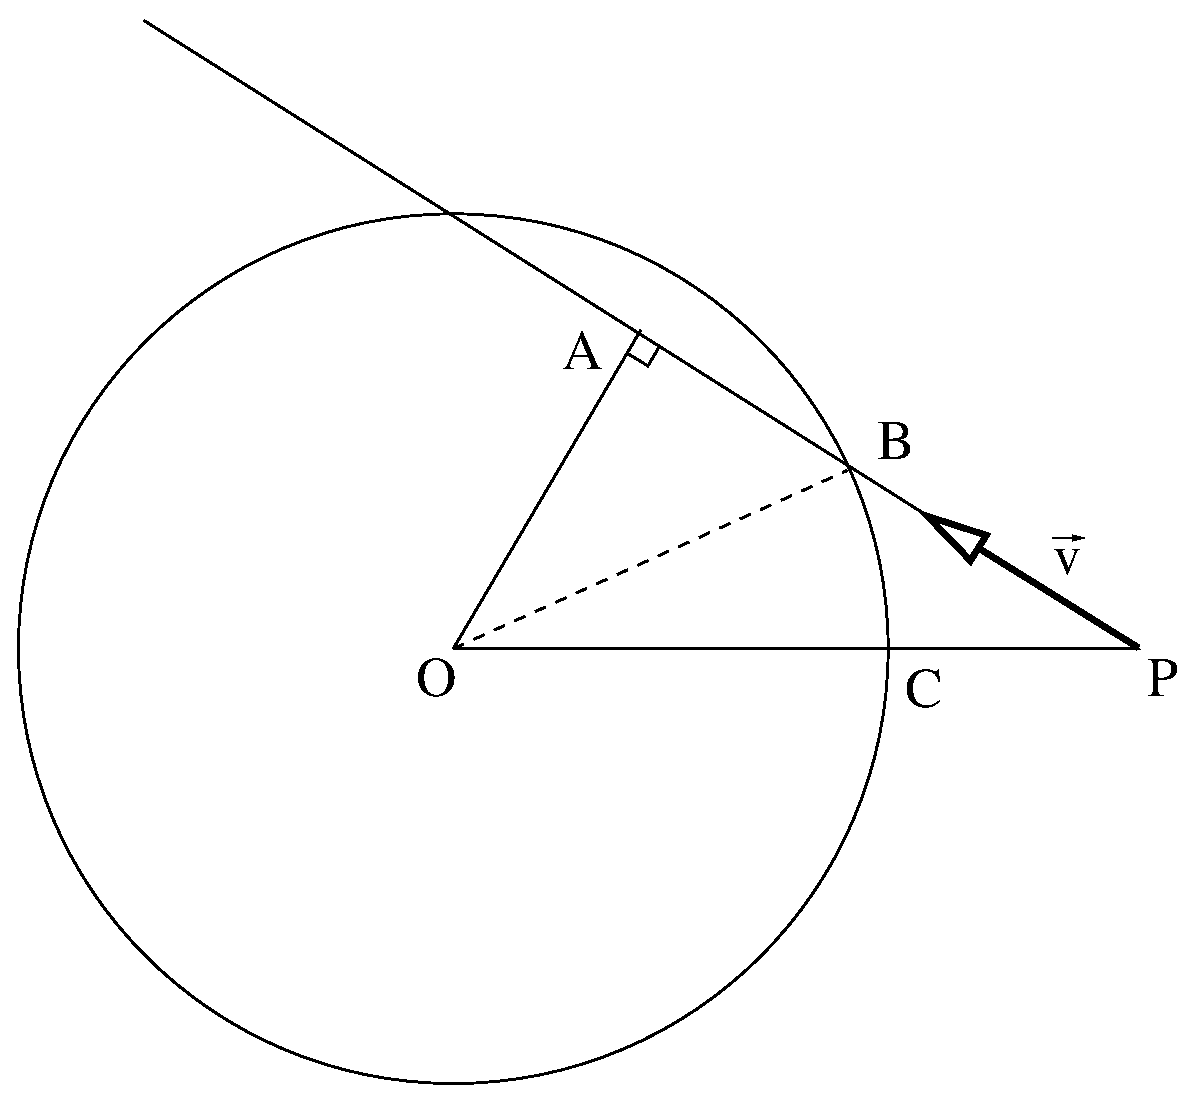
\includegraphics[width=6cm]{crpdetector.eps}
\end{center}
\caption{Geometry of a small ``observer'' sphere in \crp}
\label{fig:crpdetector}
\end{figure}

This algorithm works as long as the Larmor radius of the particle in the region of the sphere is much larger than the radius $r$ of the sphere. The accuracy of the detection algorithm is independent of the propagation time step set by the user and is of the order of $\epsilon_{1}\times\epsilon_{2}$. In the case of neutral particles the algorithm differs slightly as there is only one propagation step.

In the ``sphere around source'' case the detection algorithm is different, a particle is detected if it has crossed the sphere during the last time step. A crossing is defined as either the particle being inside the sphere at the beginning of the time step and outside of it afterwards, or vice versa. The propagation algorithm ensures that this crossing step is no larger than \verb+MinStep_Mpc+, which therefore defines the error of this detection algorithm, as in the case of a $1$D observer. 

\subsection{Performance}

We can split the running time of a typical configuration in 3 parts: a configuration independent part during which the code is initialized and cross-section tables are loaded in memory; a charged nuclei propagation part, which in general will depend on the number of injected particles (with nearly linear scaling), on the nuclear species, on the maximum propagation time and redshift of the source distribution and, in a 3D environment, also on the size of the observer(s) and on the intensity of the magnetic field; a neutral secondaries propagation part, during which basically $\gamma$-ray cascades are propagated, which takes constant time in 1D environment (thanks to the special treatment of 1D cascades described in Sec~2.2), but scales linearly with the number of cascades in a 3D environment (in fact, in 3D simulations this can take most of the running time, as charged nuclei are continuously losing energy into electron/positron pairs).

In order to have an idea of the typical performances of \crp\ we report the running time for two versions of the example \verb+examples/GettingStarted/source1d.xml+ on a standard Desktop machine (equipped with an Intel(R) Core(TM) i7-2600 CPU @ 3.40GHz, 8Mb cache).
\begin{itemize}
\item Example modified to have 1000 iron nuclei injected from a continuous source distribution extending from 3 to 4000 Mpc, in the energy range 1 - 1000 EeV, with spectral index -1. This includes propagation of secondary neutrinos and gamma rays. Execution time was 304 s.
\item Same as before, but injecting 5000 iron nuclei without neutral secondaries propagation and with minimum energy equal to 0.07 EeV. Execution time was 74 s.
\end{itemize}

\section{Inputs and outputs}

\subsection{Configuration files}

%The configuration files are written in XML are pretty self-explained. The best thing to
%do is to look at the examples/tests given on the web page.

In this section, we present the various possible ``blocks'' of XML keywords to configure a \crp\ simulation. If the XML configuration is incorrect, the execution of \crp\ will stop and an error message will explain in most cases what the problem is. However, \crp\ will not alert the user if a required block of XML is present multiple times, or an optional block is missing or misspelled. The user can find several commented example files in the \verb+examples/GettingStarted+ directory. 

\subsubsection{General parameters}

You must specify the number of particle trajectories injected at the sources
 with:

\begin{verbatim}
<TrajNumber    value=10000 />
\end{verbatim}

\noindent On most platforms, this number can be as large as 4 billion
(unsigned long). Note, that the true number of trajectories to be 
followed can be larger because all the secondaries as well as disassociated nuclei are followed once a particle has
been generated from a source. 

Use
\begin{verbatim}
<MinEnergy_EeV   value=10 />
\end{verbatim}

\noindent to determine the threshold energy below which charged
particles are abandoned. With the ``standard'' pair production table
used in the package, you can set this value to any energy above 0.07
EeV. 

Finally, the maximum propagation time after
which a particle is abandoned is set with

\begin{verbatim}
<MaxTime_Mpc    value=100 />
\end{verbatim}

\noindent Note that this time is specified in Mpc as it is
the most natural unit here. 

As an option, you can also define an integer seed
for all the random numbers in the code, which should allow to make
every simulation reproducible:

\begin{verbatim}
<RandomSeed    value = 1981 />
\end{verbatim}

The output can be of two types: the ``Full Trajectories" mode will
record charged particles at every step of their propagation, whereas
the ``Events'' mode will only record particles and secondaries which
reach an observer. The output file must be specified and the file
format can be ``ASCII'', ``FITS'' or ``ROOT''. For example you can write:

\begin{verbatim}
<Output type="Full Trajectories">
   <File type="FITS" option="force"> /My_Directory/crp_output.fits </File>
</Output>
\end{verbatim}

\noindent Note the option ``force'' which allows to overwrite an
existing file. It is also possible to switch off the output with 

\begin{verbatim}
<Output type="None" />
\end{verbatim}

 Furthermore it is possible to specify the cosmological parameters of the simulation, using: \verb+<OmegaM value=0.3 />+, \verb+<OmegaLambda value=0.7 />+, and \verb+<H0_km_s_Mpc value=65 />+. They will be used in \crp, SOPHIA and DINT. See eq. 1 of \cite{crp_paper}.

\subsubsection{Environment and magnetic field}

The environment can be either 1-Dimensional or 3-Dimensional. In the 1D case, you have to
specify

\begin{verbatim}
<Environment type="One Dimension" />
\end{verbatim}

\noindent In this case, particles are injected and propagated along the line of sight and they will be recorded (i.e.~detected) when they
reach the origin. In 3D, the only available environment at the moment is
a model for the extragalactic environment. A simulation box is used for propagation, and
periodic boundary conditions are applied: a particle that reaches a boundary reenters a copy of the original box on the opposite side. However, its coordinates are kept in the range of the original box, whereas the coordinates of its source are shifted into the new box. %It is instructive to think about the periodic boundary conditions as copies of the original simulation box.
%This allows to have
%effective sources located outside the ``main'' simulation box. Use the following definition:
The relevant XML code is the following:
\begin{verbatim}
<Environment type="LSS">
   <Xmin_Mpc value=0  />
   <Xmax_Mpc value=50 />
   (...same for Y and Z...)
</Environment>
\end{verbatim}

\noindent You must specify
the boundaries of the box only if the magnetic field is not specified elsewhere by a grid. Otherwise, the coordinate grid is taken from the magnetic field model and the user cannot specify the boundaries of the box within this tag. 

In the presence of a 3D magnetic field, you must also choose the
integrator to solve the particle's equation of motion. At the moment, a 5th order Cash-Karp RK has been implemented and is
the only available choice:

\begin{verbatim}
<Integrator type="Cash-Karp RK">
   <Epsilon value=1.e-5     />
   <MinStep_Mpc value=1.e-4 />
</Integrator>
\end{verbatim}

\noindent The Epsilon value is the accuracy on each time step. The choice of this parameter is a tradeoff between computational resources and numerical accuracy, in many cases values of the order of $10^{-4}$ are a reasonable compromise. The MinStep is an optional parameter. For step sizes smaller than \verb+MinStep_Mpc+ the RK integrator is switched off. Therefore it should be set to a value much smaller than the smallest expected Larmor radius. The default value is 10\% of the grid spacing of the magnetic field grid. 

Magnetic fields can be specified in both 1D and 3D environments.
Two simple magnetic field scenarios available are a vanishing field (``Null'') or a ``Uniform'' field. For example you can set

\begin{verbatim}
<MagneticField type="Uniform">
   <Bx_nG  value = 0  />
   <By_nG  value = 0  />
   <Bz_nG  value = 10 />
</MagneticField>
\end{verbatim}

In the case of electromagnetic cascade analysis in a 1D environment,
you can define an inhomogeneous transverse magnetic field which will
be taken into account during electromagnetic cascade development:

\begin{verbatim}
<MagneticField type="1D" >
   <File type = "ASCII" > /MyDirectory/BField_1D.txt </File>
</MagneticField>
\end{verbatim}

\noindent Currently the file format must be ASCII, and contain two
comment lines followed by an array with position(Mpc) and field($\mu$G). 

To use a 3D grid magnetic field, one must specify for example:

\begin{verbatim}
<MagneticField type="LSS-Grid">
   <Nx       value=512  />
   <Ny       value=512  />
   <Nz       value=512  />
   <Step_Mpc value=0.1  />
   <File type="FITS"> /MyDirectory/example_Bfield.fits </File>
   <Origin>
         <X_Mpc value=0 />
         <Y_Mpc value=0 />
         <Z_Mpc value=0 />
   </Origin>
</MagneticField>
\end{verbatim}

\noindent $N_x$, $N_y$ and $N_z$ are the $(x,y,z)$ sizes of the magnetic field array. At the
moment, only simple, regular-meshed arrays are implemented. The
parameter \verb+Step_Mpc+ represents the grid spacing. The file containing the grid
can be in ASCII or FITS format. In case of an ASCII file, each line must
contain the values $B_x$, $B_y$, $B_z$ in Gauss. In the
FITS case, the file must contain 3 images of size $N_x \times N_y \times
N_z$, representing in order the $B_x$, $B_y$ and $B_z$ arrays in Gauss.
An origin $\mathbf{O}$ for the magnetic field grid can also be specified in
the configuration file (default is $\mathbf{O}=(0,0,0)$).
More precisely, to calculate the trajectory of a particle at a positon
$\mathbf{x}$
the magnetic field at $\mathbf{B}(\mathbf{x}-\mathbf{O})$ is used in CRPropa.

A magnetic field with Kolmogoroff-like turbulence is also implemented. The grid parameters are the same as above, with the exception that the number of grid points needs to be the same in each direction, $N\equiv N_x=N_y=N_z$\footnote{The FFTW requires $N$ to have only prime factors smaller or equal than 13 \cite{FFTW05}. Removing the constraint of a cubic simulation box is planned for the future}. While normalization is given by the volume-averaged root mean square \verb+RMS_muG+ and the grid spacing by \verb+Step_Mpc+.


The turbulent structure itself is characterized by its maximum and minimum scales, $L_{min}$ and $L_{max}$, and by the distribution of the magnetic field energy to these scales. Since the Kolmogoroff field is produced in Fourier space it is more convenient to describe its scales in terms of wavenumbers, $\verb+Kmin+=1/L_{max}$ and $\verb+Kmax+=1/L_{min}$. The energy distribution to the different scales of the magnetic field is given by the power law index \verb+SpectralIndex+ of the expectation value of its squared Fourier transform, $\left\langle|{\bf B}({\bf k})|^2\right\rangle\propto k^{\verb+SpectralIndex+}$ in wavenumber $k$. A Kolmogoroff-spectrum in the proper sense thus corresponds to $\verb+SpectralIndex+=-11/3$. It should be noted that in the literature sometimes the spectral index of the energy density ($\text{d}E/\text{d}k\propto k^{n}$) is given, where $\verb+SpectralIndex+=n-2$.

To define this kind of magnetic field, use a block as follows:

\begin{verbatim}
<MagneticField type="Kolmogoroff">
  <Nx            value=128     />
  <Ny            value=128     />
  <Nz            value=128     />
  <Step_Mpc      value=0.3     />
  <SpectralIndex value=-3.66   />
  <RMS_muG       value=0.002   />
  <Kmin          value=0.03125 />
  <Kmax          value=0.5     />
</MagneticField>
\end{verbatim}

The magnetic field generated by CRPropa can be saved for further usage as a fits file by adding the following line to the \verb+MagneticField+ section.
\begin{verbatim}
<Outputfile option="force" name="outPutFile.fits"/>
\end{verbatim}
In this the \verb+name+ attribute is the name of the outputfile and \verb+option="force"+ indicates that the file should be overwritten, if it exists. 

Following the definitions in \cite{Harari02}, the coherence length of such a turbulent field is given by,

\begin{equation}
 L_{c}=\frac{1}{2} L_{max} \frac{n-1}{n} \frac{1- (L_{min}/L_{max})^{n}}{1- (L_{min}/L_{max})^{n-1}}
\end{equation}

The smallest possible scale is two grid points (or $\verb+Kmax+=0.5$), while the largest possible scale is given by the simulation volume (or $\verb+Kmin+=1/(N \verb+Step_Mpc+)$).

It should be noted that for all grid based magnetic field models CRPropa uses a trilinear interpolation between the gridpoints, which introduces divergences to the magnetic field \cite{Brackbill80}. While the potential error is small compared to the theoretical uncertainty of the EGMF, one should keep this in mind when comparing CRPropa simulations to exact calculations.

 Additionally it is possible to define a hydrogen gas background density. This gas density is only used for proton-proton interactions. The simplest possible gas model is spherically symmetric and can be used both in 1D and 3D simulations.
 %
 \begin{verbatim}
 <Gas type="SpherSymm">
   <File type="ASCII"> examples/variableIRandGas/n_gas.dat </File>
 </Gas>
 \end{verbatim}
 %
 The format of the ASCII file is 2 columns, containing the position in Mpc and the associated gas density in $\rm cm^{-3}$ respectively.
 
 In principle it is also possible to use a gas grid defined in the 3D space. For this one must specify for example:
 %
 \begin{verbatim}
 <Gas type="LSS-Grid">
    <Nx       value=512  />
    <Ny       value=512  />
    <Nz       value=512  />
    <Step_Mpc value=0.1  />
    <File type="FITS"> example_gas.fits </File>
 </Gas>
 \end{verbatim}
 %
 Also grids defined in plain ASCII files can be used. If magnetic fields are also defined in the simulation, then the gas grid should be the same as the one of the magnetic field model. This 3D possibility is however still experimental.


\subsubsection{Interactions}

At the moment two interaction models are implemented. The trivial one is

\begin{verbatim}
<Interactions type="None" />
\end{verbatim}
\noindent which simply switches off all interactions. 
% \noindent Proton interactions computed with tables derived from the
% DINT package are implemented with the type ``F77-proton''. They do not
% allow to generate secondary particles. 
The standard interaction type is ``Sophia''. With the ``Sophia'' interaction model, pair production is treated as a
continuous energy loss using tables derived from either DINT or the analytical expression of \cite{kelner08}. The algorithm for dialing the interaction time uses tables for the total interaction rate derived from \sophia\  for pion production and from TALYS for photodisintegration.
%Pion production is checked at each propagation step using tables derived from \sophia~itself. 
If pion production occurs, we use the \sophia\ event generator to describe the energy loss by
the proton, neutron or nuclei, as well as to get the secondary particles. In the case of nuclei, photodisintegration is taken into account using mean free path tables derived from cross sections which were calculated with the TALYS framework (for $A\geq 12$) \cite{talys}. For light, stable nuclei ($A<12$) the mean free path tables are based on fits to experimental photonuclear cross sections and parametrizations from \cite{RachenPHD,2002EPJA...14..377K,nudat2}. Additionally, the nuclear decay is treated according to the NuDat2 \cite{nudat2}, taking into account alpha decay, beta decay and nucleon dripping. By default all these processes are taken into account. 

The details of interactions are specified in an \verb+Interactions+ Block in the input file. 

\begin{verbatim}
<Interactions type="Sophia" >
   <NoPairProd /> 
   <Directory> /MySophiaTableDirectory/ </Directory>
   <MaxStep_Mpc  value=50 />
</Interactions>
\end{verbatim}

\noindent In this block the flags \verb+<NoPairProd />+, \verb+<NoPionProd />+, \verb+<NoRedshift />+, \verb+<NoPhotodisintegration />+ and \verb+<NoDecay />+\footnote{Decay implements also the \textit{nucleon dripping lines}. Therefore switching off decay may produce nuclei for which no photodisintegration is implemented.} can be used and cause the corresponding interaction to be neglected. With \verb+<NoIRO />+, pair production, pion production and photodisintegration  will be considered on the CMB only.\footnote{\texttt{<NoIRPionProd/>} is an alias for this due to compatibility to older versions of \crp.} The maximum time step for interactions has to be specified. The actual time step used by the solver of the Lorentz force varies depending on the local magnetic field but will never be larger than \verb+MaxStep_Mpc+. Additionally \verb+<PairProd_Eps value=1e-3 />+ can be used to limit the step size further. This imposes effectively a limit to the propagation step size by requiring the relative energy loss due to pair production to be smaller than $\Delta E/E < \verb+value+$ in one time step (cf.\ section \ref{propAlgo}).

 Optionally you can specify the directory where interaction tables are located. The only exception is for the photodisintegration tables which need to be located in the installation directory as specified in the \verb+configure+ procedure during the compilation of the CRPropa framework.

You can specify which kind of secondary particles you want to follow:

\begin{verbatim}
<Interactions type="Sophia" >
   <MaxStep_Mpc     value=5. />
   <SecondaryPhotons         />
   <SecondaryPairProdPhotons />
   <SecondaryNeutrinos       />
</Interactions>
\end{verbatim}


\noindent \crp\ can propagate both neutrinos and photons produced during decay and photohadronic interactions. The XML flags to configure the propagation of secondaries are:
\begin{itemize}
\item Comment in \verb+<SecondaryNeutrinos />+ and \verb+<SecondaryPhotons />+, to take into account the propagation of these neutral secondaries. 
\item \verb+<SecondaryPairProdPhotons />+ alters the behavior of the electromagnetic cascades generated by pair production. You can add a label \verb+proba=...+ to this flag if you wish only a fraction of the secondary cascades produced by pair production to be propagated (this is useful to speed-up the simulation in 3D, using a reweighting procedure in processing the output). Since CRPropa version 1.4, the secondary photons from pair production on the CMB are generated by default according to a tabulated spectrum which has been computed from the analytical work of~\cite{kelner08}. A truncated power-law may still be generated by adding the label \verb+type="PowerLaw"+ to the tag.
\end{itemize}

The \verb+<ShowerTableDirectory>+ marker can also be specified if the tables used by DINT are located in a specific directory.

\begin{figure}[htb]
\centering
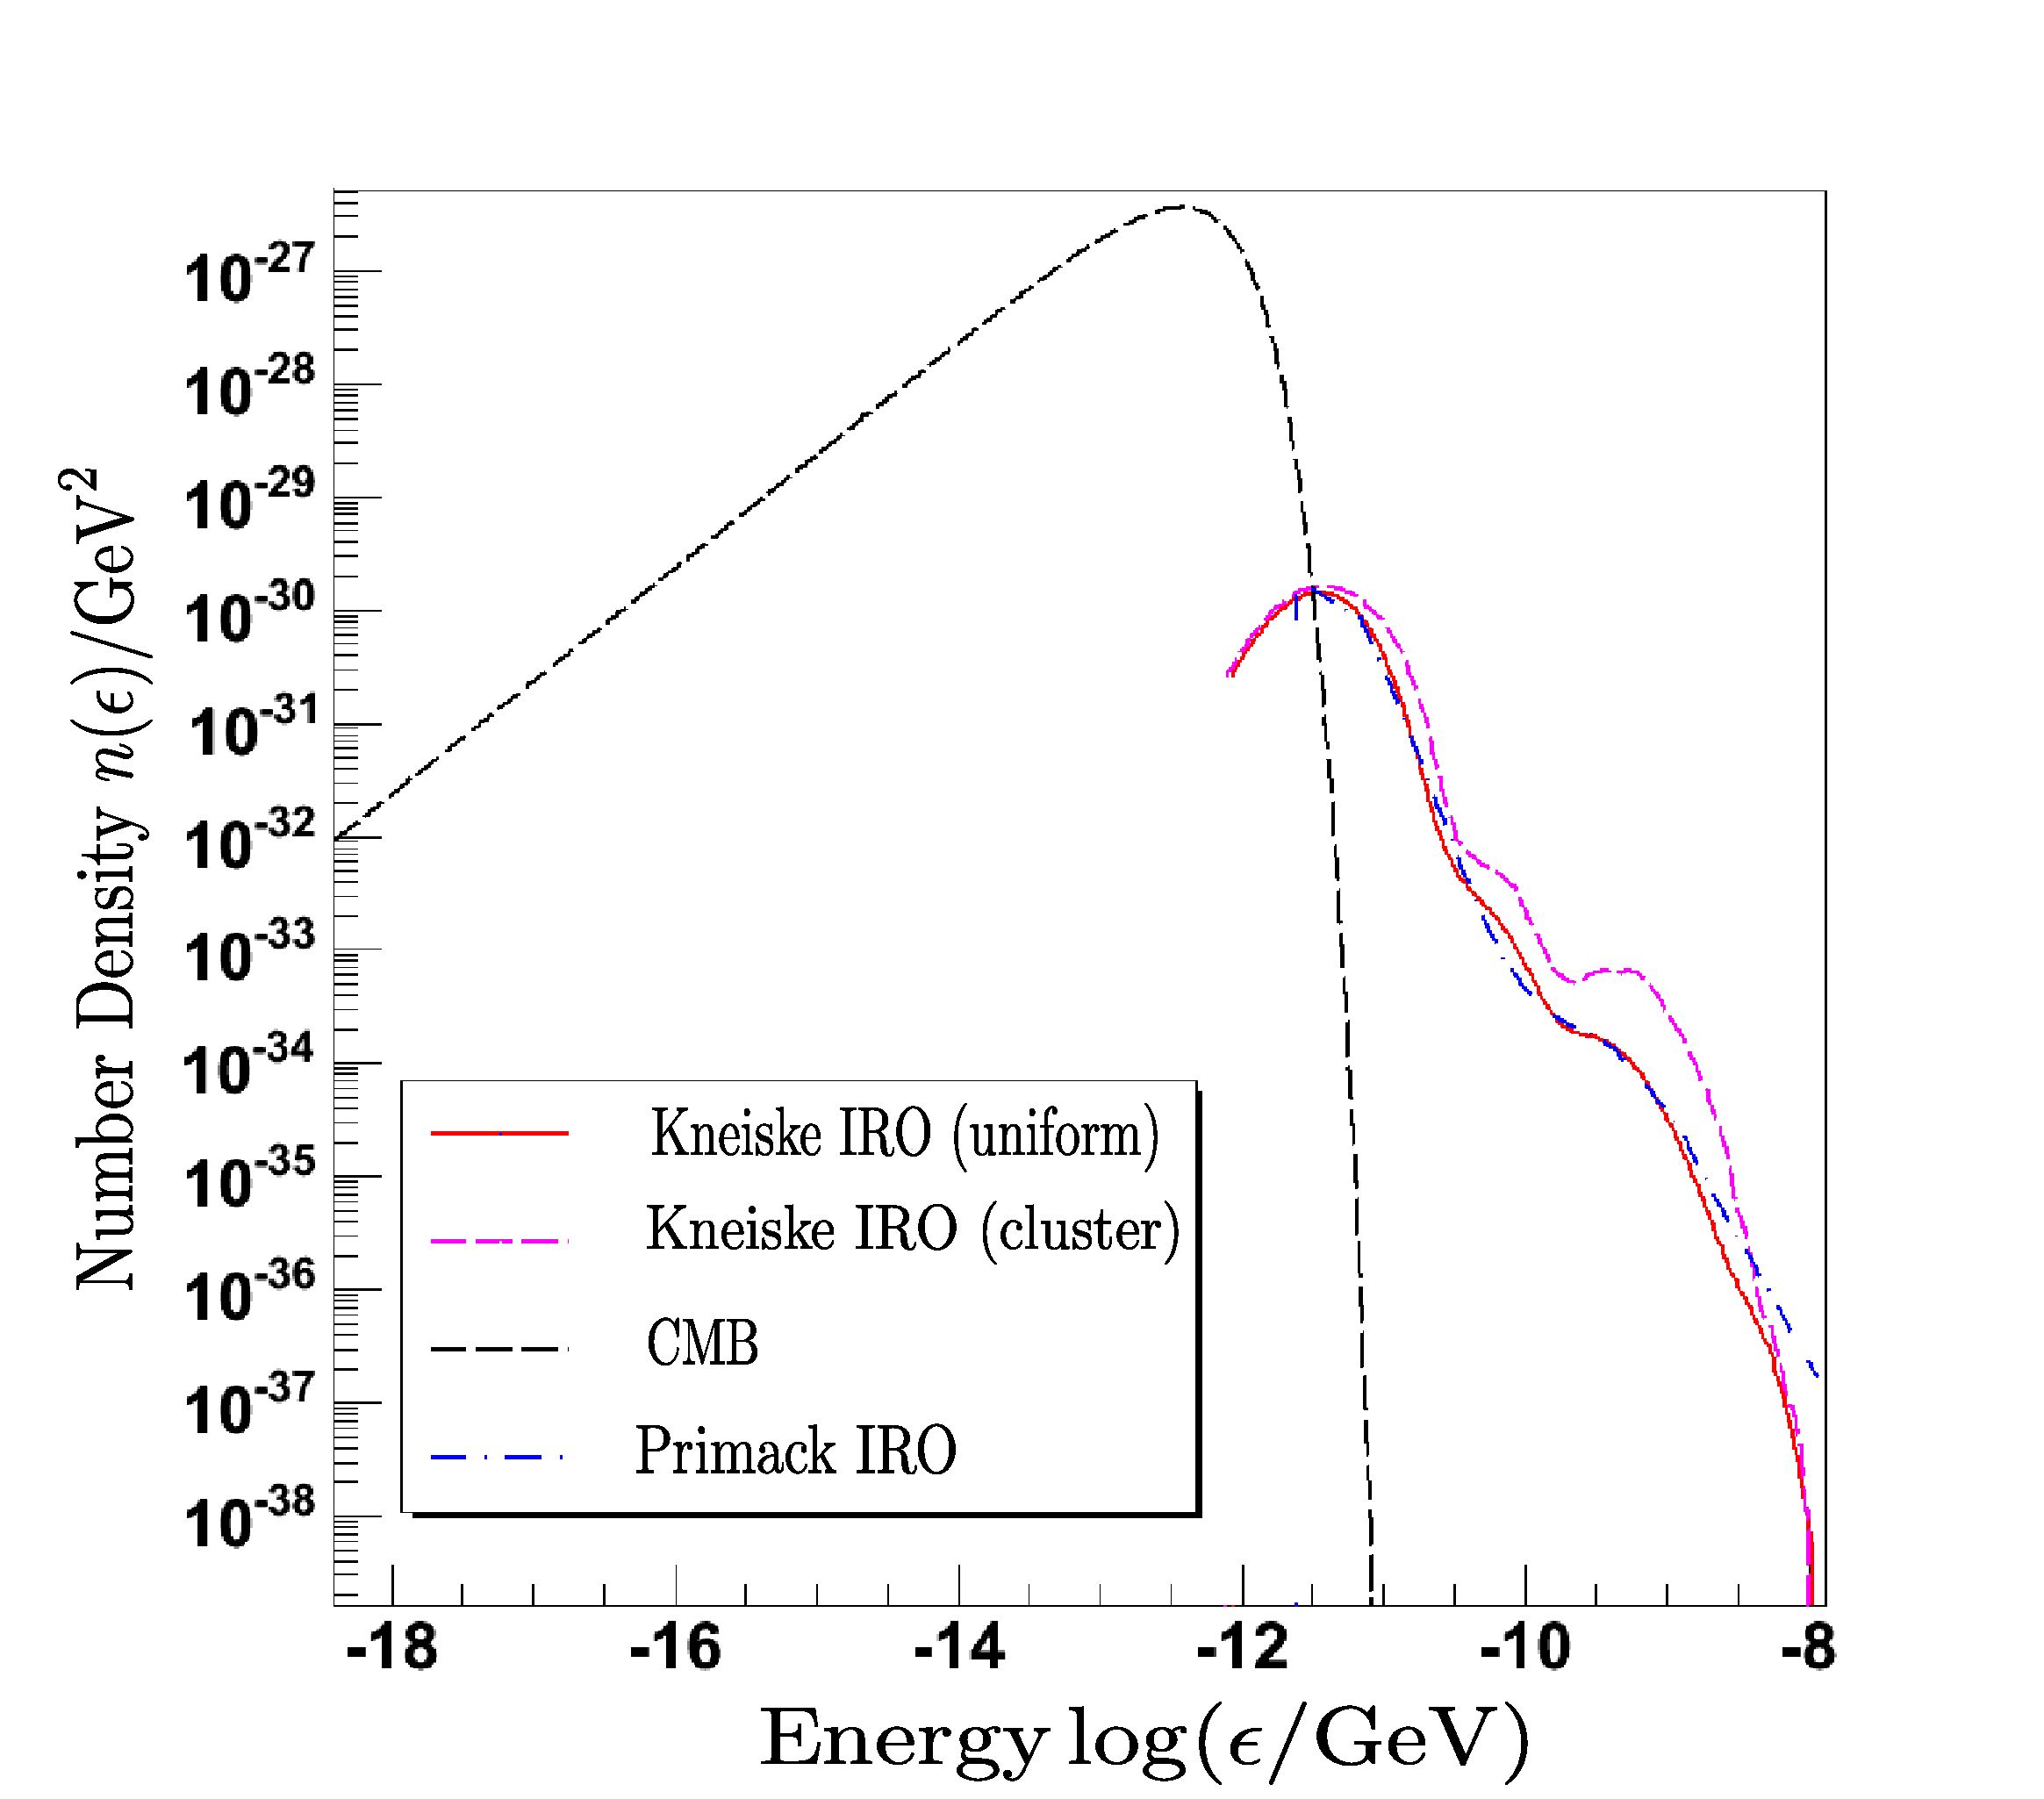
\includegraphics[scale=0.25]{PhotonDensityCollection2.eps}
\caption{EBL volume number density per photon energy. Shown is the cosmic microwave background (dashed black curve) and two different models of the uniform infrared background according to Kneiske \& al. (solid red curve) and according to \cite{Primack:2005rf} (dot-dashed blue curve). For comparison of the variability of the IRO an estimate of the IRO background in the center of a cluster is also shown (dashed magenta curve).}
\label{IROComp}
\end{figure}

\begin{figure}[tbp]
\centering
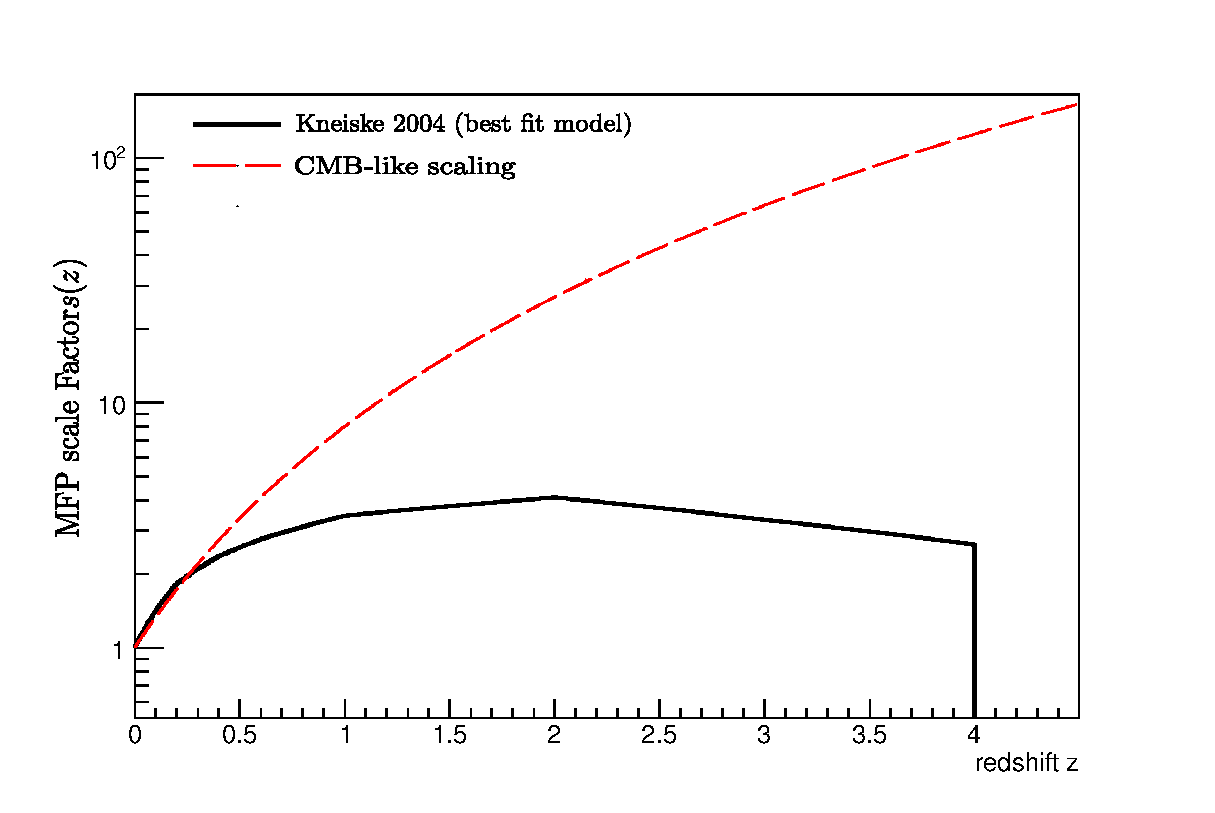
\includegraphics[scale=0.65]{AllIRBzEvolutionModelsCan.eps}
\caption{The scaling function $s_{\rm PD, \pi P}(z)$ is shown which relates the mean free path $\lambda[\Gamma, z=0]$ for an interaction with IRB photons at redshift $z=0$ with the corresponding mean free path $\lambda[\Gamma\,\,(1+z), z]$ at an earlier redshift $z$ and the Lorentz boosted $\Gamma$-factor of the nucleus. For details the reader is referred to the accompanying paper of CRPropa version 2.0.} 
\label{pic:IRB_MFPScaling}
\end{figure}

Infrared backgrounds (IRB) can be taken into account as follows:
\begin{itemize}
\item By default pion production and photodisintegration use mean free path tables derived on the basis of the extragalactic background light (EBL) at a redshift $z=0$ as parametrized by Kneiske et al., cf. figure  \ref{IROComp}. Note, that the IRB in CRPropa 1.4 was scaled like the CMB as function of the redshift $z$, cf. eq. (12) in \cite{crp_paper}, which corresponds to instantaneous production at a given redshift. Since this is not a very realistic model, in CRPropa 2.0 we alternatively provide an approximate scaling function $s(z)$ derived from Kneiske et al \cite{Kneiske:2003tx}. This function of redshift $s(z)$ is shown in fig.~\ref{pic:IRB_MFPScaling}. Furthermore the user can specify his own scaling model. This is given in a two column ascii file with redshift and scaling in the columns.
\\  Note: the ``cmb-like scaling'' up to a maximum redshift \verb+MaxRedshift+ (this corresponds to the \verb+MaxRedshift+ as defined in the \verb+<InfraredBackground>+ xml-scope explained below) is still the default option, while the alternative models can be selected via
\begin{verbatim}
<IRB_MFPScalingModel type="CMBLike" />
                     type="Kneiske2004_BestFit"
                     type="UserDefinedScaling"
                     <File type="ASCII"> ... </File>
\end{verbatim}


For the user defined scaling the same procedure as for the Kneiske model is applied with the possibility to provide a scaling model externally. In the file the deviation from the CMB scaling is given, thus a file containing just ones is identical to CMBLike scaling. 
In the case of \verb+None+ a constant scale function $s(z)=1$ is applied which corresponds to the non-physical case of no scaling.


\item The DINT package calculates the development of electromagnetic cascades in the IRB. It takes into account reactions in the CMB, IRB and universal radio background (URB). For the IRB it uses by default the same IRB as is used for calculations of UHECR interactions, see figure \ref{IROComp}. In addition there are also "high" and "low" flags aviable, which switch the IRB model for DINT only to models based on \cite{Franceschini:2001yg}, compare \cite{crp_paper} for details. This can be usefull for simulations in which the production of electromagnetic cascades is not strongly affected by the IRB, while the shape of the cascade at TeV energies is. In DINT it is possible to switch off the reactions with IRB photons for redshifts larger than \verb+<MaxRedshift>+. The same IRB model is also used in \sophia\ for the production of neutral secondaries from photopion interactions. 

\begin{verbatim}
<InfraredBackground type="Uniform">
   <SpectralShape type="Kneiske" />
   <MaxRedshift   value=3        />
</InfraredBackground>
\end{verbatim}
The model of the URB used in cascade development can be chosen with  
\verb+<RadioBackground+ \verb+type="Obs" />+. 
The available options are \verb+Obs+, \verb+Med+, \verb+High+ and \verb+Null+.

\item A new feature in this version is the propagation of nucleons in variable IRB photon backgrounds.
\begin{verbatim}
<InfraredBackground type="Variable" >
  <SpectralShape type="Shells" />
  <MaxRedshift   value=0.0     />
  <File type="ASCII"> IR_table.data </File>
</InfraredBackground>
\end{verbatim}
 Note, that the variable IRB option is not available for nuclei ($A>1$) in this version of CRPropa. This major improvement will be presumably included in a later version.
\end{itemize}

For protons it is further possible to calculate hadronic interactions with ambient proton gas by specifying \verb+<PPProd />+. For this a background gas density must be given.

Keep in mind, that the \verb+InfraredBackground+ XML block is outside of the \verb+Interactions+ block. 
% The low-energy photon backgrounds and the cosmological parameters can be optionally specified. For example:

% \begin{verbatim}
% <InfraredBackground type="Uniform">
%    <SpectralShape type="Primack" />
%    <MaxRedshift   value=3 />
% </InfraredBackground>
% \end{verbatim}

% \noindent This will use a Primack-like IR background with a redshift evolution as described in~\cite{crp_paper}, until a given redshift. No inhomogeneous IR background can be used for nuclei propagation yet. The only model used at the moment is from Kneiske \& al. 
% %IR background spectral shapes can be "Primack", "High" or "Low" (refering to models described in~\cite{crp_paper}). 
% You can also specify a \verb+<RadioBackground >+, with types "High", "Med", "Obs" or "Null" as described again in~\cite{crp_paper}. The default radio background is "Obs". The following cosmological parameters can be set: \verb+<OmegaM value=0.3 />+, \verb+<OmegaLambda value=0.7 />+, and \verb+<H0_km_s_Mpc value=65 />+. They will be used in \crp, SOPHIA and DINT.
% For pionproduction on protons only it is possible to define a variable infrared background as 
% \begin{verbatim}
% <InfraredBackground type="Variable" >
%   <SpectralShape type="Shells" />
%   <MaxRedshift value = 0.0 />
%   <File type="ASCII"> IR_table.data </File>
% </InfraredBackground>
% \end{verbatim}

Even in three dimensions the development of secondary electromagnetic cascades is calculated in a straight-line approximation. This is only valid if electrons and positrons are not strongly deflected in EGMF. How well this approximations works, can be tested in a given configuration by adding the \verb+<CutCascade_MagField />+ marker within the \verb+<Interactions>+ block. In this case, within DINT, the electron/positron spectrum of the cascade below a critical energy $E_c$ is set to zero at each step of the cascade development. Here, $E_c$ is the energy below which deflections are faster than energy losses. Thus, if the usage of \verb+<CutCascade_MagField />+ strongly effects the resulting photon spectra in your simulations, you should reconsider the usage of the rectilinear approximation in 3D. Note, $E_c$ depends on a dimensionless parameter $A$ and is linked to an angular deflection of the e+/e- pairs, see  page 6 in \cite{crp_paper} for details. $A$ can be changed by adding the label \verb+value=...+ to the \verb+<CutCascade_MagField />+ marker (the default value of A is 1).

%To conclude, it is possible in 1D to study the propagation of EM cascades only (that is to use CRPropa as a simple interface to the DINT module). To do so, one must specify the marker \verb+<Particles type="Photons"/>+ inside the \verb+<Sources>+ block. In the interaction block, you have to specify for example:

%\begin{verbatim}
%<Interactions type="Photon" >
%   <CutCascade_MagField value=10 />
%</Interactions>
%\end{verbatim}


\subsubsection{Sources and observers}

Charged particle sources can be of two types: ``Continuous'' or
``Discrete''. 
\begin{description}
\item[Continuous] sources must be defined with a space
density. The initial position of a charged particle is then randomly
computed from the density, in 1D or 3D. 
\item[Discrete] sources can be
directly defined with a list of coordinates, or can also be defined by
a space density and a fixed number of sources N. In that case, N
sources are drawn at the beginning of the simulation from the 1D or 3D
space density.
\end{description}

The source spectra are of two kinds: ``Monochromatic'' (you must then
define the energy), or ``Power Law'' (in this case, you have to define
a maximal energy/rigidity and spectral index $\alpha$, such that the injection spectra is $\sim E^{-\alpha}$). Here are two examples of source definitions in the XML files:

\begin{verbatim}
<!-- 1D Continuous monochromatic source density -->
<Sources type="Continuous">
   <Density type="Grid">
      <File type="ASCII"> /MyDirectory/Density_1D_Model.txt </File>
      <Nx         value=2000 />
      <Step_Mpc   value=0.1  />
   </Density>
   <Spectrum type="Monochromatic">
      <Energy_EeV value=100  />
   </Spectrum>
</Sources>

<!-- A single source in 3D with a power law spectrum -->
<Sources type="Discrete">
   <Number value=1 />
   <PointSource>
      <CoordX_Mpc value=10.87 />
      <CoordY_Mpc value=20.12 />
      <CoordZ_Mpc value=43.45 />
   </PointSource>
   <Spectrum type="Power Law">
      <Ecut_EeV   value=300   />
      <Alpha      value=2.2   />
   </Spectrum>
</Sources>
\end{verbatim}

\noindent ASCII density files must begin with two lines of comments,
followed by density values on a regular grid (density can be given in arbitrary units). In 1D, the scaling with redshift should be given as comoving density. In 3D, you can use FITS files containing a single $Nx \times Ny
\times Nz$ image. You can also specify a uniform density with \verb+<Density type="Uniform">+, and the associated boundaries \verb+<Xmin_Mpc value=0 />+, etc.  

\crp{ }can also determine a list of source positions at random from a given source distribution. In this case the sources block of the simulation should contain \verb+Discrete+ sources and the \verb+Number+ of sources as well as the definition of a density distribution.

\begin{verbatim}
<!-- 5 sources with source positions determined from a 
uniform source distribution. --> 
<Sources type="Discrete">
   <Number value=5 />
   <Density type="Uniform">
      <Xmin_Mpc value=0  />
      <Xmax_Mpc value=10 />
      <Ymin_Mpc value=0  />
      <Ymax_Mpc value=10 />
      <Zmin_Mpc value=0  />
      <Zmax_Mpc value=10 />
   </Density>
<!-- In this simulation an equal number of trajectories per logarithmic bin is 
injected up to a maximum rigidity E/A= 100 EeV -->
   <Spectrum type="Power Law">
      <Alpha        value=1    />
      <Rigidity_EeV value=1.e2 />
   </Spectrum>
</Sources>
\end{verbatim}
Additionally the sources block contains the specification of the injection spectra. The maximum possible energy that can be propagated is $E_{\rm max}=A\cdot 10^{22}$~eV for nuclei with mass number $A$. In addition, trajectories may be injected up to a specified rigidity \verb+Rigidity_EeV+ instead of maximal energy \verb+Ecut_EeV+. 

\begin{verbatim}
<Spectrum type="Power Law">
   <Alpha        value=2   />
   <Rigidity_EeV value=500 />
</Spectrum>
\end{verbatim}
This works also for \verb+<Spectrum type="Monochromatic">+.

Furthermore, a source composition needs to be specified in the \verb+Sources+ block. For example:
\begin{verbatim}
<Particles type="Nuclei">
   <Number_Of_Species value=3 />
   <Species MassNumber=56 ChargeNumber=26 Abundance=10 />
   <Species MassNumber=24 ChargeNumber=12 Abundance=10 />
   <Species MassNumber=1  ChargeNumber=1  Abundance=10 />
</Particles>
\end{verbatim}
In this example the three species, Iron ($^{56}$Fe), Magnesium ($^{24}$Mg) and protons are injected with equal abundance. If a maximum energy is defined the flag \verb+Abundance+ refers to a given energy or equivalently to the abundance integrated over all energies. For a maximum rigidity \verb+Abundance+ refers to a constant energy per nucleon, $E/A$. For one species only it is also possible to specify mass and charge like
\begin{verbatim}
<Particles type="Nuclei">
  <MassNumber   value=1 />
  <ChargeNumber value=1 />
</Particles>
\end{verbatim}

In 1D also primary photons can be injected. This can be achieved by setting\\ \verb+<Particles type=Photons>+.

Observers must be defined if the output type is ``Events'' and the
simulation is in 3D (in 1D, the observer is simply a point at $x =
0$). Two kinds of observers are implemented in 3D:

\begin{enumerate}
\item{``Spheres around Source''. In this case, you must have only
one discrete source. The center of the observers must be at the same
location as the source, and you can specify observers of various
radii. Charged particles are recorded each time they go through one of
the spheres. If you include secondary photons or neutrinos, only one
observer can be defined. As an example:

\begin{verbatim}
<Observers type="Spheres around Source">
   <Number value=1 />
   <Sphere>
      <CoordX_Mpc value=35.0 />
      <CoordY_Mpc value=20.0 />
      <CoordZ_Mpc value=10.0 />
      <Radius_Mpc value=40.0 />
   </Sphere>
</Observers>
\end{verbatim}

}
\item{``Spheres around Observers''. Observers are defined by small
spheres; a particle is recorded each time it enters the observer sphere. The size of the sphere should not be too large, so as to make
the observer as point-like as possible, but the smaller the sphere the
smaller the detection efficiency.

\begin{verbatim}
<Observers type="Spheres around Observers">
   <Number     value=1   />
   <Radius_Mpc value=1.5 />
   <SphereObserver>
      <CoordX_Mpc value=41.85 />
      <CoordY_Mpc value=55.80 />
      <CoordZ_Mpc value=5.580 />
   </SphereObserver>
</Observers>
\end{verbatim}

}
\end{enumerate}


\subsection{Output files}

In ASCII, FITS or ROOT, the output files are tables (binary tables in FITS, Ntuples or TTrees in ROOT) whose formats
differ depending on the configuration.

\begin{itemize}
\item{{\bf 1D Full trajectories.} Each line or NTuple has 5 fields: 
\center{Particle\_Type Initial\_Particle\_Type Time Position Energy}

}
\item{{\bf 3D Full trajectories.}} Each line or NTuple has the fields: 
\begin{center} Particle\_Type Initial\_Particle\_Type Time Position[X,Y,Z] Momentum[X, Y, Z](EeV) Energy \end{center}

Furthermore, each trajectory starts with a line containing the
fields: -1, -1, -1, source position (x,y,z), -1. This provides the possibility to
determine what the source of the particle is. This can be crucial information as the position is given relative to the source. Additionally the energy is given in EeV and the particle type is defined as $Z + A \times 1000$, with mass number $A$ and charge number $Z$. Therefore, $^{56} \rm Fe$ is labeled as 26056. 

\item{{\bf 1D Charged particle events.} Fields: 
\center{Particle\_Type Initial\_Particle\_Type Initial\_Position(Mpc) Initial\_Energy(EeV) Time(Mpc) Energy(EeV)
}
In case of a root output file there is an additional field \verb+Inital_Redshift+ with the redshift at injection. 
}
\item{{\bf 3D Charged particle events.} Fields:
\center{ Particle\_Type Initial\_Particle\_Type Initial\_Position[X,Y,Z](Mpc)\\ Initial\_Momentum[E, $\theta$, $\phi$](EeV) Time(Mpc) Position[X,Y,Z](Mpc) Momentum[E, $\theta$ ,$\phi$](EeV)}

The particle position will always be inside the simulation box, but
not the initial position. This is a consequence of the periodic boundary conditions.
}
\item{{\bf 1D Neutrinos.} Fields:

\center{ Particle\_Type Generating\_Particle Source\_Position(Mpc) Initial\_Position(Mpc) Initial\_Energy(EeV) Energy(EeV) Source\_Energy(EeV)}

The source position and energy correspond to the source and initial energy of the charged
particle which generated the neutrino. The initial position and energy correspond to the
state of the neutrino when is was created by an interaction. The Generating\_Particle field contains the type of the generating nucleus at the source. 
}
\item{{\bf 3D Neutrinos.} Fields:
\center{ Particle\_Type Generating\_Particle Source\_Position[X,Y,Z](Mpc) Initial\_Position[X,Y,Z](Mpc) Position[X,Y,Z](Mpc) Momentum[E,$\theta$ ,$\phi$](EeV) Source\_Energy(EeV)}

For neutrinos in three dimensions it should be noted that the initial position is always inside the simulation box, while the source position and the detected position may be outside of this box. 
}

\item{{\bf 1D electromagnetic shower.} For electromagnetic showers,
the full cascade spectrum is recorded. There are 170 energy bins for
this spectrum (10 bins per decade, ranging from 100 MeV to $10^{25}$ eV). The spectrum represents the mean number of particles per energy bin (which are logarithmically
distributed). In the ASCII case, 170 rows are recorded. In the FITS
case, the output file contains a binary table extension with seven fields per row. In the ROOT case, a TTree is used (instead of simple NTuples for other particles).
The positions of the energy bins are given in the file. 
\begin{enumerate}
\item{In case of an ASCII or FITS output: The first line of the table has the same format, but instead of the shower spectrum, the numerical values for the 170 shower energy bins are given. Therefore do not forget to remove the first line of the table before you start to analyze the secondary spectrum.}
\item{In case of a ROOT output: there is an additional "SpectrumEnergy" leaf in the TTree.}
\end{enumerate}

 The fields are:
\begin{center} Particle\_type Cascade\_Origin Source\_position Initial\_Position  Energy  Source\_Energy  Shower\_Spectrum(170 bins)\end{center}

 In the  case of 1D propagation, the electromagnetic cascades from a given point are propagated only once (compare page \pageref{1dphotons}) and their origin is therefore marked as ``1D\_ALL'' and the Energy and Source\_Energy fields are ``0''.

}

\item{{\bf 3D electromagnetic shower.} Identical with the fields:
\center{ particle type - cascade origin - initial type - source position(x,y,z) - initial
position(x,y,z) - position(x,y,z) - momentum(energy,$\theta$,$\phi$) -
source energy - shower spectrum(170 bins)}

The field "cascade origin" is a flag to recognize which interaction generated the cascade. It is a 10 character long string delimited by white space for ASCII and fits output. The cascade can be generated from the decay products of $\pi$ decay, photons \verb+pi_gamma+, positrons \verb-pi_e+- or electrons \verb+pi_e-+. Additionally pair production \verb+PairProd+ and $\beta$ decays can initiate an electromagnetic cascade. In case of $\beta$ decay the origin string is \verb+A:XZ:Yb-+, where \verb+X+ and \verb+Z+ denote mass and charge of the decaying nucleus and the \verb+-+ denotes the type of the $\beta^\pm$ decay. The energy is the full shower energy, i.e. the energy of the primary photon/electron/positron if the cascade was generated by a GZK interaction, or the energy lost by a proton during pair production over a given time $\Delta t$. The source energy is the energy of the generating nucleus at the source, this is usefull to change the injection spectra after the simulation by adding energy-dependend weights.
}
\end{itemize}

%The particle type is always a 10 character string: \verb+pp+, \verb+n+,
%\verb+neutrino+, \verb+gamma+, \verb+e++, \verb+e-+,
%\verb+gamma_pair+ (for a cascade generated by pair production).

%The particle type is always an integer using the HEP PDT code: 2212 for protons, 2112 for neutrons, 22 for photons, 12 for $\nu_{e}$, -12 for $\tilde{\nu}_e$, 14 for $\nu_{\mu}$ and -14 for $\tilde{\nu}_{\mu}$. 


\section{Plotting routine}
\crp\ version 2.0 is accompanied by plotting routines meant to help the user understanding \crp\ output. The plotting routines use \ROOT~extensively. The routines can:
\begin{itemize}
\item plot \crp\ output files normalized to the Auger spectrum~\cite{augerspec} and the spectrum of secondaries if available. Additionally it can reweigh the spectrum to a different injection index;
\item plot distributions of deflection angles, maps of arrival directions, possibly with true sources if provided (this may require the use of the IDL package).
\end{itemize}

The routines depend on \cfitsio\footnote{included in the \crp\ External directory, if you installed \crp\ using {\tt get\_external.sh}.} for reading fits files and Healpix~\cite{healpix} for skymaps. 

\subsection{How to...}
To use the plotting routines, you first need to configure \ROOT~appropriately. In particular, you must tell \ROOT{ }where to find the \cfitsio~and Healpix libraries and include files. This can be done by putting in your plotting directory (from where you launch the plotting routines) a file named \verb+.rootlogon.C+ (notice the initial ``dot''). A possible  \verb+.rootlogon.C+ can look like the following:
%
\begin{verbatim}
{
gSystem->SetIncludePath("-I$ROOTSYS/include 
    -I$SOFTWAREDIR/Healpix_2.20a/include/ -I$SOFTWAREDIR//cfitsio/include");
gSystem->AddLinkedLibs("$SOFTWAREDIR/cfitsio/lib/libcfitsio.a");
gSystem->AddLinkedLibs("-L$SOFTWAREDIR/Healpix_2.20a/lib -lchealpix");
//gSystem->AddLinkedLibs("$SOFTWAREDIR/Healpix_2.20a/lib/libchealpix.a");
gSystem->Load("libGeom.so");
}
\end{verbatim}
% 
% \begin{verbatim}
% {
% gSystem->SetIncludePath("-I$ROOTSYS/include 
% -I/home/yoshi/CRPropa/Healpix_2.15a/include/ 
% -I../External/cfitsio/include");
% gSystem->AddLinkedLibs("../External/cfitsio/lib/libcfitsio.a");
% gSystem->AddLinkedLibs("/home/yoshi/CRPropa/Healpix_2.15a/lib/libchealpix.a");
% gSystem->Load("libGeom.so");
% }
% \end{verbatim}
%
After this, the user can start \ROOT~and compile the library by typing
%
\begin{verbatim}
.L utils.cc+
.L crpropaoutput.cc+
.L plot_spectrum.cc+
.L plot_deflections.cc+
\end{verbatim}
%
into the \ROOT~shell. Then you can plot the spectra of cosmic rays and secondaries with the function \verb+plot_spectrum()+, which in the simplest case is called as 
%
\begin{verbatim}
plot_spectrum(file, norm_en, spect_ind, old_spec)
\end{verbatim}
%
where \verb+file+ points to a single output file of \crp, or to an entire directory. \verb+norm_en+ is the normalization energy of the spectrum and the other two parameters, \verb+spect_ind+ and \verb+old_spec+ control reweighting of the spectrum from a simulation with spectral index \verb+old_spec+ to a spectrum \verb+spect_ind+. Notice that it is not possible to reweight a $\gamma$-ray spectrum in 1D, because of the way in which it is propagated within \crp.

% \begin{tabular}{l|l|l}
% section & XML Flag & Notes\\
% \hline
% \hline
% General & & \\
% \end{tabular}

\begin{thebibliography}{999}
\bibitem{crp2paper} Karl-Heinz Kampert, J\"org Kulbartz, Luca Maccione, Nils Nierstenhoefer, Peter Schiffer, G\"unter Sigl, Arjen René van Vliet arXiv:1206.3132 [astro-ph.IM]

\bibitem{crp_paper} E.~Armengaud, G.~Sigl, T.~Beau and F.~Miniati, Astropart. Phys. 28/4-5 pp.463-471 (2007) [arXiv:astro-ph/0603675]
\bibitem{crp_paper2_ICRC09} ,``Propagation of Ultra-High Energy Nuclei with CRPropa'', K.-H.~Kampert et. al., In \textit{Proceedings of the 31$^{\rm st}$ ICRC 2009} 
\bibitem{kelner08}
   S.~R.~Kelner and F.~A.~Aharonian,
  %``Energy spectra of gamma-rays, electrons and neutrinos produced at
  %interactions of relativistic protons with low energy radiation,''
  Phys.\ Rev.\  D {\bf 78}, 034013 (2008)
%  [arXiv:0803.0688 [astro-ph]].
  %%CITATION = PHRVA,D78,034013;%%
%\cite{Primack:2005rf}
\bibitem{Primack:2005rf}
  J.~R.~Primack, J.~S.~Bullock and R.~S.~Somerville,
  %``Observational gamma-ray cosmology,''
  AIP Conf.\ Proc.\  {\bf 745} (2005) 23
  [arXiv:astro-ph/0502177].
  %%CITATION = APCPC,745,23;%%
\bibitem{numrec} \url{http://www.library.cornell.edu/nr/bookcpdf.html}
\bibitem{RachenPHD} {Rachen}, J., \textit{Interaction Processes and Statistical Properties of the Propagation of Cosmic Rays in Photon Backgrounds}, Universitat zu Bonn, 1996.
\bibitem{Lee:1996fp}
  S.~Lee,
  %``On the propagation of extragalactic high-energy cosmic and gamma-rays,''
  Phys.\ Rev.\ D {\bf 58}, 043004 (1998)
  [arXiv:astro-ph/9604098].
  %%CITATION = ASTRO-PH 9604098;%%
\bibitem{sophia}
  A.~Mucke, R.~Engel, J.~P.~Rachen, R.~J.~Protheroe and T.~Stanev,
  %``Monte Carlo simulations of photohadronic processes in astrophysics,''
  Comput.\ Phys.\ Commun.\  {\bf 124}, 290 (2000)
%  [arXiv:astro-ph/9903478].
  %%CITATION = ASTRO-PH 9903478;%
  \bibitem{Ahn:2009wx}
  E.~-J.~Ahn, R.~Engel, T.~K.~Gaisser {\it et al.},
  %``Cosmic ray interaction event generator SIBYLL 2.1,''
  Phys.\ Rev.\  {\bf D80 } (2009)  094003.
  [arXiv:0906.4113 [hep-ph]].
\bibitem{tinyxml} {\url{http://www.grinninglizard.com/tinyxml/}}
\bibitem{2002EPJA...14..377K}  M.~V.~{Kossov},\textit{Approximation of photonuclear interaction cross-sections}, European Physical Journal A, 2002, 14, 377-392.
\bibitem{cfitsio} {\url{http://heasarc.gsfc.nasa.gov/docs/software/fitsio/}}
\bibitem{clhep} {\url{http://www.cern.ch/clhep/}}
\bibitem{root} {\url{http://root.cern.ch/}}
\bibitem{talys} {\url{http://www.talys.eu/}}
\bibitem{nudat2} {\url{http://www.nndc.bnl.gov/nudat2/}}
\bibitem{healpix}{\url{http://healpix.jpl.nasa.gov/}}
\bibitem{augerspec}{F.~Sch\"ussler for the Pierre Auger Collaboration, 
ICRC 2009 Proceedings 
{\url{http://www.auger.org/technical\_info/ICRC2009/arxiv\_spectrum.pdf}}}
\bibitem{Kneiske:2003tx}
  T.~M.~Kneiske, T.~Bretz, K.~Mannheim and D.~H.~Hartmann,
  %``Implications of cosmological gamma-ray absorption. 2. Modification of gamma-ray spectra,''
  Astron.\ Astrophys.\  {\bf 413} (2004) 807
  [astro-ph/0309141].
  %%CITATION = ASTRO-PH/0309141;%%
\bibitem{FFTW05}{Matteo Frigo and Steven G. Johnson, Proceedings of the IEEE 93 (2), 216–231 (2005). \url{http://www.fftw.org/}}
%\cite{Franceschini:2001yg}
\bibitem{Franceschini:2001yg}
  A.~Franceschini, H.~Aussel, C.~J.~Cesarsky, D.~Elbaz and D.~Fadda,
  %``A long-wavelength view on galaxy evolution from deep surveys by the infrared space observatory,''
  Astron.\ Astrophys.\  {\bf 378} (2001) 1
  [astro-ph/0108292].
  %%CITATION = ASTRO-PH/0108292;%%
\bibitem{Harari02}
  D.~Harari, S.~Mollerach, E.~Roulet,
  %``A long-wavelength view on galaxy evolution from deep surveys by the infrared space observatory,''
  Journal of High Energy Physics, {\bf 03}, 045 (2002).  
  [astro-ph/0202362v2].
\bibitem{Brackbill80}
  J.U.~Brackbill, D.C.~Barnes,
Journal of Computational Physics, {\bf 35}, 3, 426–430 (1980).


\end{thebibliography}

\section*{Appendix: Available markers in the configuration files}

We list here all the currently possible markers for the XML files.

\begin{verbatim}
<TrajNumber    value=... />
<MinEnergy_EeV value=... />
<MaxTime_Mpc   value=... />
<RandomSeed    value=... />

<Output type="None">
        type="Full Trajectories"
        type="Events"
   <File option="force" type="ASCII"> ... </File>
                        type="FITS"
                        type="ROOT"
</Output>

<InfraredBackground type="Uniform" >
   <SpectralShape type="Kneiske" />
                  type="Low"
                  type="High"
   <MaxRedshift value=... />
<InfraredBackground type="Variable" >
   <SpectralShape type="Shells" />
   <MaxRedshift value=... />
   <File type="ASCII"> ... </File>
</InfraredBackground>

<RadioBackground type="High" />
                 type="Med"
                 type="Obs"
                 type="Null"

<IRB_MFPScalingModel type="CMBLike" />
                     type="Kneiske2004_BestFit"
                     type="UserDefinedScaling"
   <File type="ASCII"> ... </File>

<OmegaM      value=... />
<OmegaLambda value=... />
<H0_km_s_Mpc value=... />

<Interactions type="None" />
<Interactions type="Sophia" >
    <Directory> ... </Directory>
    <MaxStep_Mpc value=... />
    <NoRedshift            />
    <NoPairProd            />
    <NoPionProd            />
    <NoIRPionProd          />
    <NoIRO                 />
    <NoPhotodisintegration />
    <NoDecay               />
    <SecondaryPhotons      />
    <SecondaryPairProdPhotons proba=... />
    <SecondaryPairProdPhotons type="PowerLaw" proba=... />
    <SecondaryNeutrinos    />
    <CutCascade_MagField value=... />
    <ShowerTableDirectory> ... </ShowerTableDirectory>
    <PPProd                />
    <PairProd_Eps        value=... />
</Interactions>

<Environment type="One Dimension" />
<Environment type="LSS" >
    <Xmin_Mpc value=... />
    <Xmax_Mpc value=... />
    <Ymin_Mpc value=... />
    <Ymax_Mpc value=... />
    <Zmin_Mpc value=... />
    <Zmax_Mpc value=... />
</Environment>

<MagneticField type="Null" />
<MagneticField type="1D">
    <File type="ASCII"> ... </File>
<MagneticField type="Uniform">
    <Bx_nG value=... />
    <By_nG value=... />
    <Bz_nG value=... />
<MagneticField type="LSS-Grid">
    <Nx       value=... />
    <Ny       value=... />
    <Nz       value=... />
    <Step_Mpc value=... />
    <Origin>
         <X_Mpc value=... />
         <Y_Mpc value=... />
         <Z_Mpc value=... />
    </Origin>
    <File type="ASCII"> ... </File>
          type="FITS"
<MagneticField type="Kolmogoroff">
   <Nx            value=... />
   <Ny            value=... />
   <Nz            value=... />
   <Step_Mpc      value=... />
   <SpectralIndex value=... />
   <RMS_muG       value=... />
   <Kmin          value= .../>
   <Kmax          value= .../>
</MagneticField>

<Gas type="SpherSymm">
   <File type="ASCII"> ... </File>
</Gas>

<Integrator type="Cash-Karp RK">
    <Epsilon     value=... />
    <MinStep_Mpc value=... />
</Integrator>

<Sources type="Discrete">
         type="Continuous"
    <Number value=... />
    <PointSource>
         <CoordX_Mpc value=... />
         <CoordY_Mpc value=... />
         <CoordZ_Mpc value=... />
    </PointSource>

    <Density type="Uniform">
         <Xmin_Mpc value=... />
         <Xmax_Mpc value=... />
         <Ymin_Mpc value=... />
         <Ymax_Mpc value=... />
         <Zmin_Mpc value=... />
         <Zmax_Mpc value=... />
    <Density type="Grid" >
         <Nx       value=... />
         <Ny       value=... />
         <Nz       value=... />
         <Step_Mpc value=... />
         <Origin>
              <X_Mpc value=... />
              <Y_Mpc value=... />
              <Z_Mpc value=... />
         </Origin>
         <File type="ASCII"> ... </File>
               type="FITS"
    </Density>

    <Spectrum type="Monochromatic">
         <Energy_EeV   value=... />
         <Rigidity_EeV value=... />  
    <Spectrum type="Power Law">
         <Alpha        value=... />
         <SigmaAlpha   value=... />
         <Ecut_EeV     value=... />
         <Rigidity_EeV value=... />
    </Spectrum>
    <Particles type="Nuclei">
         <Number_Of_Species value=... />
         <Species MassNumber=... ChargeNumber=... Abundance=... />
    </Particles>
</Sources>

<Observers type="Spheres around Observer">
           type="Spheres around Source"
    <Number     value=... />
    <Radius_Mpc value=... />
    <Sphere>
         <CoordX_Mpc value=... />
         <CoordY_Mpc value=... />
         <CoordZ_Mpc value=... />
         <Radius_Mpc value=... />
    </Sphere>
    <SphereObserver>
         <CoordX_Mpc value=... />
         <CoordY_Mpc value=... />
         <CoordZ_Mpc value=... />
    </SphereObserver>
</Observers>

\end{verbatim}

\end{document}
